\documentclass[aps,pra,twocolumn,superscriptaddress,nofootinbib]{revtex4-2}

\usepackage{amsmath,amssymb,mathtools,bm}
\usepackage{booktabs}
\usepackage{tabularx}
\usepackage[hidelinks]{hyperref}
\usepackage{xcolor}
\usepackage{microtype}

\newcommand{\ii}{\mathrm{i}}
\newcommand{\eff}{\mathrm{eff}}
\newcommand{\B}{\mathrm{B}}
\newcommand{\g}{\mathrm{g}}
\newcommand{\rt}{\mathrm{rt}}
\newcommand{\env}{\mathrm{env}}
\newcommand{\tot}{\mathrm{tot}}
\newcommand{\res}{\mathrm{res}}
\newcommand{\dd}{\mathrm{d}}
\renewcommand{\Re}{\operatorname{Re}}
\renewcommand{\Im}{\operatorname{Im}}

\begin{document}

\title{Reflection Phase of Uniform and Chirped Fiber Bragg Gratings}
\author{NanoQT}
\date{\today}

\begin{abstract}
We clarify the reflection phase of uniform and chirped fiber Bragg gratings in the context of FBG cavities. 
For a uniform grating, the Bloch phase is pinned inside the stop band, so the Bragg-period carrier only shifts the longitudinal mode index.
The observable dispersion instead arises from the bounded boundary, or envelope, phase and does not scale with the number of grating periods. 
In contrast, chirped gratings exhibit a frequency-dependent reflection point, producing the designed group delay.
\end{abstract}

\maketitle

\section{Introduction}

A field propagating a geometric distance $L$ in a homogeneous medium accumulates the phase $kL$.  This intuition can be misleading for reflection from a fiber Bragg grating (FBG).  A uniform FBG may contain $10^3$--$10^5$ periods, but the reflection phase across the stop band changes only by order $\pi$ rather than by the many-thousand-$\pi$ phase one might associate with the physical grating length.  At the same time, different frequencies penetrate to different effective depths before being reflected.  The purpose of this note is to separate these two statements and make clear which phase is observable in a cavity.

The central point is a change of basis.  Near the Bragg condition the field is written as a rapidly varying Bragg carrier multiplied by slowly varying forward and backward envelopes.  Equivalently, the unit-cell transfer matrix is diagonalized into Bloch eigenmodes.  For a uniform grating inside the stop band, the real Bloch phase is fixed at the Brillouin-zone edge, $\Re(\theta)=\pi$, while the imaginary part sets the evanescent decay.  Therefore the large carrier phase is constant across the stop band.  The frequency-dependent reflection phase comes from boundary matching between the external waves and the evanescent Bloch modes.

We keep the main text at the level needed for cavity design.  Appendix~\ref{app:uniform} gives the coupled-mode formulas for a uniform FBG, Appendix~\ref{app:tmm} gives the transfer-matrix diagonalization, and Appendix~\ref{app:wkb} gives the WKB derivation for chirped gratings.  Standard treatments of these results can be found in Refs.~\cite{Erdogan1997,OthonosKalli1999,Kashyap2009,YarivYeh1984,Joannopoulos2008}.

\section{Uniform FBG: phase decomposition}
\label{sec:uniform}

Consider a lossless uniform FBG with period $\Lambda$, length $L=N\Lambda$, and Bragg wave vector
\begin{equation}
    \beta_\B=\frac{\pi}{\Lambda}.
\end{equation}
Near the Bragg frequency, the electric field may be written as
\begin{equation}
    E(z)=A(z)e^{\ii\beta_\B z}+B(z)e^{-\ii\beta_\B z},
\end{equation}
where $A$ and $B$ are slowly varying envelopes.  The rapidly varying factor $e^{\pm\ii\beta_\B z}$ is the Bragg carrier.  The reflection coefficient referred to the input face is
\begin{equation}
    r(\omega)=\frac{B(0)}{A(0)},\qquad \phi_r(\omega)=\arg r(\omega).
\end{equation}
Thus $\phi_r$ is already an envelope phase: the carrier has been factored out by the choice of basis.

The same statement appears in transfer-matrix form.  
Let $M$ be the transfer matrix of one period.  For a lossless periodic structure (see the details in Appendix \ref{app:tmm} and Eq.(\ref{eq:tmat_def})),
\begin{equation}
    M=O\Lambda_M O^{-1},\qquad
    \Lambda_M=\begin{pmatrix} e^{\ii\theta} & 0\\ 0 & e^{-\ii\theta}\end{pmatrix},
\end{equation}
where $\theta=\beta\Lambda$ is the Bloch phase per period.  For $N$ periods,
\begin{equation}
    M^N=O\Lambda_M^N O^{-1}.
\end{equation}
The factor $\Lambda_M^N$ is the Bragg carrier in the Bloch basis; the matrices $O$ and $O^{-1}$ are boundary-matching operators, which contribute to the side-lobe of the FBG spectra for finite length structure.

Inside the stop band, the Bloch phase can be written as
\begin{equation}
    \theta=\pi+\ii\theta_i(\omega),\qquad \theta_i\ge 0.
    \label{eq:stopband_theta}
\end{equation}
Therefore
\begin{equation}
    \Lambda_M^N=\begin{pmatrix}
    e^{\ii N\pi}e^{-N\theta_i} & 0\\
    0 & e^{-\ii N\pi}e^{N\theta_i}
    \end{pmatrix}.
\end{equation}
The real part of the carrier is the constant phase $N\pi$.  It does not vary with frequency inside the stop band.  The frequency dependence of the reflection phase comes from the boundary operators $O$ and $O^{-1}$ and from the finite penetration of the evanescent Bloch mode.

For a strong uniform grating, the reflected phase changes by approximately $\pi$ across the stop band.  In coupled-mode notation, with detuning $\delta=\beta(\omega)-\beta_\B$ and coupling coefficient $\kappa$, the semi-infinite grating has
\begin{equation}
    r_\infty(\omega)=\frac{\delta-\ii\sqrt{\kappa^2-\delta^2}}{\kappa},
    \qquad |\delta|<\kappa,
    \label{eq:r_infty}
\end{equation}
up to an overall convention-dependent constant phase.  Equation~\eqref{eq:r_infty} has unit magnitude and its phase winds by $\pi$ as $\delta$ crosses the gap.  The finite-length expression and sign conventions are given in Appendix~\ref{app:uniform}.

The reflected-field group delay, for the convention used here, is
\begin{equation}
    \tau_g(\omega)=-\frac{\dd\phi_r}{\dd\omega},
    \label{eq:tau_def}
\end{equation}
which defines the effective penetration depth
\begin{equation}
    L_\eff^{\rm FBG}(\omega)=\frac{v_g\tau_g(\omega)}{2}
    =-\frac{v_g}{2}\frac{\dd\phi_r}{\dd\omega}.
    \label{eq:Leff_def}
\end{equation}
At the center of a strong uniform grating,
\begin{equation}
    L_\eff^{\rm FBG}(\omega_\B)=\frac{\tanh(\kappa L)}{2\kappa}
    \longrightarrow \frac{1}{2\kappa}\qquad (\kappa L\gg 1),
    \label{eq:Leff_center}
\end{equation}
where $v_g$ is the group velocity of the unperturbed guided mode.  The increase of $L_\eff$ near the stop-band edges comes from the derivative of the envelope phase, not from a frequency-dependent carrier phase.

\section{FBG cavities}
\label{sec:cavity}



Now consider two uniform FBGs facing each other and separated by a physical gap $L_{\rm gap}$.  The resonance condition may be written as
\begin{equation}
    \Phi_{\rm rt}(\omega)=2k(\omega)L_{\rm gap}
    +\phi_{r,1}(\omega)+\phi_{r,2}(\omega)=2\pi m.
    \label{eq:rt_phase}
\end{equation}
If the two FBGs are operated inside their common stop band, each reflection phase can be decomposed schematically as
\begin{equation}
    \phi_{r,j}(\omega)=N_j\pi+\phi_{{\rm env},j}(\omega),
    \label{eq:cavity_decomp}
\end{equation}
where $N_j\pi$ is the frequency-independent carrier contribution, including any fixed reference-plane convention, and $\phi_{{\rm env},j}$ is the bounded envelope phase.  Substitution into Eq.~\eqref{eq:rt_phase} gives
\begin{equation}
    2k(\omega)L_{\rm gap}+\phi_{{\rm env},1}(\omega)+\phi_{{\rm env},2}(\omega)
    =2\pi m',
\end{equation}
with $m'=m-(N_1+N_2)/2$ up to a constant parity convention.  Thus the Bragg carrier only relabels the longitudinal mode index.  It does not affect the resonant frequencies, free spectral range, penetration depth, or group delay.

Differentiating Eq.~\eqref{eq:rt_phase} gives the effective cavity length,
\begin{equation}
    L_{\rm cav}^\eff(\omega)=L_{\rm gap}
    +L_{\eff,1}^{\rm FBG}(\omega)+L_{\eff,2}^{\rm FBG}(\omega),
    \label{eq:cavity_length_general}
\end{equation}
which for two identical mirrors reduces to
\begin{equation}
    L_{\rm cav}^\eff=L_{\rm gap}+2L_\eff^{\rm FBG}.
\end{equation}
Because $L_\eff^{\rm FBG}$ is proportional to $\dd\phi_r/\dd\omega$, the constant $N\pi$ carrier gives exactly zero contribution.

Two qualifications are important.  First, outside the stop band the Bloch phase $\theta(\omega)$ is real and frequency dependent, so $N\theta(\omega)$ behaves like an ordinary propagation phase through the grating.  The cancellation above is specific to operation inside the stop band.  Second, the imaginary part $N\theta_i(\omega)$ in Eq.~\eqref{eq:stopband_theta} is physically important: it determines the reflectivity magnitude and therefore the finesse and linewidth.  It does not, however, provide an additional real round-trip phase.

\section{Chirped FBGs}
\label{sec:chirped}

For a chirped FBG, the period and local Bragg wave vector depend on position,
\begin{equation}
    \Lambda\rightarrow \Lambda(z),\qquad
    \beta_\B(z)=\frac{\pi}{\Lambda(z)}.
\end{equation}
There is no exact global Bloch phase.  If the chirp is slow on the scale set by the coupling, a local coupled-mode or WKB description is appropriate.  For a frequency inside the chirp-swept reflection band, the turning point $z_B(\omega)$ is defined by
\begin{equation}
    \delta(\omega,z_B)=\beta(\omega)-\beta_\B(z_B)=0,
    \label{eq:turning_point}
\end{equation}
up to the usual finite-gap correction that the reflection occurs over a distance of order $1/\kappa$.

With the group-delay sign convention of Eq.~\eqref{eq:tau_def}, the leading WKB reflection phase is
\begin{equation}
    \phi_r(\omega)\simeq
    -2\int_0^{z_B(\omega)}[\beta(\omega)-\beta_\B(z)]\,\dd z+\phi_{\rm tp},
    \label{eq:wkb_phase}
\end{equation}
where $\phi_{\rm tp}$ is a convention-dependent turning-point phase, often written as a Maslov phase of magnitude $\pi/2$.  The sign of $\phi_{\rm tp}$ and any constant offset depend on the definition of $r$ and of the reference plane; its derivative is usually negligible for group-delay design.

Taking the derivative of Eq.~\eqref{eq:wkb_phase}, the moving-boundary term vanishes because the detuning is zero at $z_B$.  For weak material dispersion over the grating bandwidth,
\begin{equation}
    \tau_g(\omega)=-\frac{\dd\phi_r}{\dd\omega}
    \simeq 2\frac{\dd\beta}{\dd\omega}z_B(\omega)
    =\frac{2z_B(\omega)}{v_g}.
    \label{eq:chirped_delay}
\end{equation}
This is the main design rule for chirped FBGs: the group delay maps frequency to the physical turning point.  For linear chirp, this gives
\begin{equation}
    \frac{\dd\tau_g}{\dd\lambda}
    \simeq \frac{2}{v_g}\left(\frac{\dd\lambda_B}{\dd z}\right)^{-1}_{z=z_B},
    \label{eq:chirped_dispersion}
\end{equation}
which is the standard inverse-chirp-rate scaling.

This behavior is qualitatively different from a uniform FBG cavity.  In a chirped grating, the upper limit $z_B(\omega)$ is frequency dependent, so the accumulated local Bragg phase cannot be reduced to a constant mode-index shift.  The frequency-dependent turning point is precisely what produces the designed group-delay dispersion.

\section{Summary}

The useful design distinction is the following.  In a uniform FBG operated inside its stop band, the real Bloch phase is pinned at $\pi$ per period.  The large Bragg carrier therefore contributes only a frequency-independent phase.  Reflection-phase dispersion, penetration depth, and cavity FSR are governed by the bounded envelope phase.  In a chirped FBG, translational symmetry is intentionally broken; the local turning point moves with frequency, and the WKB phase integral gives the designed group delay.

For FBG cavities this means that one should model each uniform FBG mirror by its complex reflection coefficient referred to a fixed reference plane.  The constant carrier phase may be absorbed into the longitudinal mode number, while the derivative of the envelope phase gives the effective mirror penetration depth.  This is the self-consistent reason why standard Fabry--P\'erot formulas with
\begin{equation}
    L_{\rm cav}^{\eff}=L_{\rm gap}+L_{\eff,1}^{\rm FBG}+L_{\eff,2}^{\rm FBG}
\end{equation}
remain valid even when each FBG contains many thousands of Bragg periods.

\appendix

\section{Uniform coupled-mode formulas}
\label{app:uniform}
This appendix summarizes the coupled-mode formulation used to describe the reflection phase of a uniform fiber Bragg grating.
Let the forward and backward envelopes obey
\begin{align}
    \frac{\dd A}{\dd z}&=\ii\delta A+\ii\kappa B,\\
    \frac{\dd B}{\dd z}&=-\ii\delta B-\ii\kappa A,
    \label{eq:cmt}
\end{align}
where $\delta=\beta(\omega)-\beta_\B$ and $\kappa$ is real.  The stop band is $|\delta|<\kappa$, and
\begin{equation}
    \gamma=\sqrt{\kappa^2-\delta^2}.
\end{equation}
For a grating of length $L$ with no incident wave from the far side, $B(L)=0$, the reflection coefficient at $z=0$ is
\begin{equation}
    r_L(\omega)=\frac{-\ii\kappa\sinh(\gamma L)}{
    \gamma\cosh(\gamma L)-\ii\delta\sinh(\gamma L)}.
    \label{eq:r_finite}
\end{equation}
Different sign conventions for Eq.~\eqref{eq:cmt} multiply $r_L$ by a constant phase or replace $\delta\rightarrow-\delta$.  These changes do not affect the physical group delay after the convention is fixed.

At exact Bragg resonance, $\delta=0$, Eq.~\eqref{eq:r_finite} gives $r_L=-\ii\tanh(\kappa L)$.  Expanding $\arg r_L$ around $\delta=0$ yields
\begin{equation}
    \tau_g(\omega_B)=-\frac{\dd\arg r_L}{\dd\omega}
    =\frac{\tanh(\kappa L)}{\kappa v_g},
\end{equation}
which gives Eq.~\eqref{eq:Leff_center}.

For $\kappa L\gg1$, Eq.~\eqref{eq:r_finite} approaches Eq.~\eqref{eq:r_infty}, up to the same constant phase convention:
\begin{equation}
    r_\infty(\omega)=\frac{\delta-\ii\sqrt{\kappa^2-\delta^2}}{\kappa},
    \qquad |r_\infty|=1.
\end{equation}
The phase changes by $\pi$ between the two band edges.

\section{Transfer-matrix diagonalization}
\label{app:tmm}

For a reciprocal lossless unit cell, the transfer matrix can be written as~\cite{Markos2008, 1dfbgnote}
\begin{equation}
\label{eq:tmdef}
M = \begin{pmatrix} 1/t^* & r/t \\ r^*/t^* & 1/t \end{pmatrix},
\qquad |t|^2+|r|^2=1,
\qquad \det M=1.
\end{equation}
Its eigenvalues are $e^{\pm\ii\theta}$, where
\begin{equation}
    \cos\theta=\frac{1}{2}\operatorname{Tr}[M]=\Re\left(\frac{1}{t}\right).
\end{equation}
The stop band corresponds to $|\Re(1/t)|>1$.  Near the first Bragg gap we choose the branch $\theta=\pi+\ii\theta_i$, which pins $\Re\theta=\pi$ and makes $\theta_i$ the evanescent decay per unit cell.

One possible eigenvector parametrization is
\begin{equation}
    s=\frac{\sin\theta}{|r/t|},\qquad
    f=\sqrt{1+s^2}-s,
    \qquad e^{\ii\varphi}=\ii e^{\ii\arg(r/t)}.
\end{equation}
Then the diagonalizing matrix may be written, up to normalization, as
\begin{equation}
    \label{eq:tmat_def} O=\begin{pmatrix}1&e^{\ii\varphi}f\\ e^{-\ii\varphi}f&1\end{pmatrix},
    \qquad M=O\begin{pmatrix}e^{\ii\theta}&0\\0&e^{-\ii\theta}\end{pmatrix}O^{-1}.
\end{equation}
Inside the stop band $s$ is imaginary and $|f|=1$ away from the band-edge singularity of this parametrization.  The phase of $f$ is the bounded envelope phase that appears as the reflection phase of a semi-infinite periodic medium.  At the gap center it is shifted by $\pi/2$ relative to the band edge, consistent with the coupled-mode result above.

For $N$ periods,
\begin{equation}
    M^N=O\begin{pmatrix}e^{\ii N\theta}&0\\0&e^{-\ii N\theta}\end{pmatrix}O^{-1}.
\end{equation}
Outside the stop band, $\theta$ is real and the finite grating exhibits transmission resonances when $N\theta=m\pi$.  Inside the stop band, $\Re(N\theta)=N\pi$ is constant and $\Im(N\theta)=N\theta_i$ controls the exponential suppression of transmission.

\section{WKB estimate for a chirped grating}
\label{app:wkb}

For slowly varying $\beta_B(z)$ and $\kappa(z)$, the coupled-mode equations can be treated locally.  The local detuning is
\begin{equation}
    \delta(\omega,z)=\beta(\omega)-\beta_B(z).
\end{equation}
The local stop-band edge occurs when $|\delta|\sim\kappa$; in the simplified turning-point estimate used in the main text we set $\delta=0$ to define $z_B(\omega)$.  A more accurate estimate replaces $z_B$ by the appropriate edge of the local forbidden region and adds a penetration correction of order $1/\kappa(z_B)$.

The WKB reflection phase has the form
\begin{equation}
    \phi_r(\omega)\simeq -2\int_0^{z_B(\omega)}\delta(\omega,z)\,\dd z+\phi_{\rm tp}.
\end{equation}
Differentiating gives
\begin{equation}
    -\frac{\dd\phi_r}{\dd\omega}
    =2\int_0^{z_B}\frac{\partial\delta}{\partial\omega}\,\dd z
    +2\delta(\omega,z_B)\frac{\dd z_B}{\dd\omega}
    -\frac{\dd\phi_{\rm tp}}{\dd\omega}.
\end{equation}
The second term vanishes at the turning point.  If $\partial\delta/\partial\omega\simeq1/v_g$ and the turning-point phase is slowly varying, Eq.~\eqref{eq:chirped_delay} follows.

The WKB condition is that the chirp be slow on the coupling length,
\begin{equation}
    \left|\frac{\dd\beta_B}{\dd z}\right|\ll \kappa^2,
\end{equation}
with the local $\kappa(z)$ used for apodized gratings.  If this condition is not satisfied, the full piecewise-uniform transfer-matrix calculation should be used.


% \section{Geometry and parameters}
% \label{sec:geometry}

% The simulated cavity has three contiguous segments along the propagation axis
% $z$:
% \begin{enumerate}\setlength\itemsep{2pt}
%   \item \textbf{FBG1}: chirped grating of total length
%         $L_\mathrm{FBG} = \sum_{j=1}^{N_\mathrm{cell}} a_j$, occupying
%         $z \in [0,\;L_\mathrm{FBG}]$. The local lattice constant $a_j$ is the
%         chirp profile saved as \texttt{a\_in} in the source HDF5; the index
%         modulation envelope $\delta n(z)$ is reconstructed from the embedded
%         \texttt{settings} JSON.
%   \item \textbf{Waveguide}: uniform medium of refractive index
%         $n_\mathrm{wg}$ and length $L_\mathrm{wg}$, with optional fractional
%         intensity loss $\eta$ per pass. Occupies
%         $z \in [L_\mathrm{FBG},\;L_\mathrm{FBG}+L_\mathrm{wg}]$.
%   \item \textbf{FBG2}: identical chirped grating (symmetric cavity).
%         Occupies $z \in [L_\mathrm{FBG}+L_\mathrm{wg},\;2L_\mathrm{FBG}+L_\mathrm{wg}]$.
% \end{enumerate}

% The defaults in the \texttt{\_\_main\_\_} block of
% \texttt{fbg\_cavity\_analysis.py} are
% \begin{equation}
%   \nu_0 = c/(1389\,\mathrm{nm}),\quad
%   L_\mathrm{wg} = 10\,\mathrm{mm},\quad
%   n_\mathrm{wg} = 1.454,\quad
%   \eta = 0,
% \end{equation}
% where $\nu_0$ matches the FBG resonance set in \texttt{gen\_fbg\_data.py} and
% $n_\mathrm{wg}$ is matched to the FBG background index $n_0$.

% \section{Intra-cavity intensity reconstructions}
% \label{sec:cascade}

% Each segment is described by a $2\times 2$ transfer matrix $M$ acting on the
% forward/backward complex amplitudes
% $\mathbf{v}(z) \equiv (E_+(z),\,E_-(z))^\top$. Following the convention used
% in \texttt{fbg.py}, every elementary unit cell has the structure
% $M = \begin{pmatrix} a^* & b \\ b^* & a \end{pmatrix}$ (preserved under
% multiplication, $\det M = 1$ for lossless cells), and the observed scattering
% of a slab characterised by $M$ is read off as
% \begin{equation}
%   t = \frac{1}{M_{11}}, \qquad
%   r = \frac{M_{10}}{M_{11}}.
%   \label{eq:tr_M}
% \end{equation}

% \paragraph{FBG block from saved $(t, r)$.}
% Inverting Eq.~\eqref{eq:tr_M} under the structure constraint gives the four
% entries directly in terms of the observed scattering data:
% \begin{equation}
%   M_\mathrm{FBG}(\nu)
%   \;=\;
%   \begin{pmatrix}
%     1/t^*(\nu) & r(\nu)/t(\nu) \\
%     r^*(\nu)/t^*(\nu) & 1/t(\nu)
%   \end{pmatrix},
%   \label{eq:M_FBG}
% \end{equation}
% implemented in \texttt{fbg\_transfer\_matrix}. This lets us reuse the heavy
% single-FBG simulation (saved on a fine detuning grid by
% \texttt{gen\_fbg\_data.py}) without redoing the per-cell transfer-matrix
% chain.

% \paragraph{Waveguide.}
% Pure propagation by $L_\mathrm{wg}$ at index $n_\mathrm{wg}$ with optional
% intensity loss $\eta$ per pass:
% \begin{equation}
%   M_\mathrm{wg}(\nu)
%   \;=\;
%   \begin{pmatrix}
%     e^{-i\phi_\mathrm{wg}}\sqrt{1-\eta} & 0 \\
%     0 & e^{+i\phi_\mathrm{wg}}/\sqrt{1-\eta}
%   \end{pmatrix},
%   \qquad
%   \phi_\mathrm{wg} \equiv \frac{2\pi\nu\,n_\mathrm{wg}\,L_\mathrm{wg}}{c}.
%   \label{eq:M_wg}
% \end{equation}
% The asymmetric scaling $\sqrt{1-\eta}$ vs.\ $1/\sqrt{1-\eta}$ keeps
% $\det M_\mathrm{wg} = 1$, so reciprocity is preserved while unitarity is
% broken (\texttt{waveguide\_transfer\_matrix}).

% \paragraph{Cavity scattering.}
% The cavity matrix is the cascade
% \begin{equation}
%   M_\mathrm{cav}(\nu)
%   \;=\;
%   M_\mathrm{FBG}(\nu)\,M_\mathrm{wg}(\nu)\,M_\mathrm{FBG}(\nu),
%   \label{eq:M_cav}
% \end{equation}
% and the cavity scattering follows from Eq.~\eqref{eq:tr_M}:
% \begin{equation}
%   t_\mathrm{cav}(\nu) \;=\; \frac{1}{M_{\mathrm{cav},11}(\nu)},
%   \qquad
%   r_\mathrm{cav}(\nu) \;=\; \frac{M_{\mathrm{cav},10}(\nu)}{M_{\mathrm{cav},11}(\nu)}.
% \end{equation}
% This is the \texttt{cavity\_t\_r} routine, vectorised over $\nu$ via
% \texttt{numpy} broadcasting.

% \section{Locating cavity resonances}
% \label{sec:peaks}

% Cavity resonances are local maxima of $|t_\mathrm{cav}(\nu)|^2$. With the
% default \texttt{detuning\_point}$=500\,000$ over a 200~GHz span, the saved
% grid spacing is
% \begin{equation}
%   df \;=\; \frac{200\,\mathrm{GHz}}{500\,000} \;\approx\; 0.4\,\mathrm{MHz},
% \end{equation}
% which is far finer than the typical cavity FWHM. The peak finder is therefore
% just a one-shot \texttt{scipy.signal.find\_peaks} call on the saved
% spectrum:
% \begin{verbatim}
% T = np.abs(t_cav) ** 2
% mask = (detuning >= -100*GHz) & (detuning <= 100*GHz)
% peaks, _ = find_peaks(T[mask],
%                       prominence=0.01 * T[mask].max(),
%                       distance=int(2*GHz / df))
% peak_idx = np.flatnonzero(mask)[peaks]
% peak_det = detuning[peak_idx]
% \end{verbatim}
% The resonance frequencies are then exactly $\{\nu_0 + \mathtt{detuning}[k]\}_k$,
% and the matched complex scattering data at those peaks are obtained by direct
% indexing,
% $t_\mathrm{cav}^{(p)} = t_\mathrm{cav}[\mathtt{peak\_idx}]$ and
% $r_\mathrm{cav}^{(p)} = r_\mathrm{cav}[\mathtt{peak\_idx}]$.
% Frequency error $\le df/2 \approx 0.2\,\mathrm{MHz}$ and amplitude error
% $\sim (df/\mathrm{FWHM})^2$ are both negligible for the cavities of interest.
% The legacy refinement routine \texttt{find\_cavity\_resonances} is retained
% in the module for use with coarser saved grids.

\section{Intracavity-field reconstruction}
\label{sec:intracavity}

\subsection{Boundary condition}
We consider unit incident amplitude from the left and no input from the right. 
The field vector at the input plane is therefore fixed as
\begin{equation}
  \mathbf{v}(0)
  =
  \begin{pmatrix} E_+(0) \\ E_-(0) \end{pmatrix}
  =
  \begin{pmatrix} 1 \\ -r_\mathrm{cav}(\nu) \end{pmatrix},
  \label{eq:bc}
\end{equation}
where $r_\mathrm{cav}(\nu)$ is the cavity reflection coefficient. The sign of the backward component follows from the transfer-matrix convention in Eq.~\eqref{eq:tmdef}, ensuring zero outgoing left-moving amplitude at the right boundary.

\subsection{Field reconstruction via transfer matrices}
The intracavity field is obtained by propagating $\mathbf{v}$ through the structure using transfer matrices. For any segment of length $\ell$ with transfer matrix $M_\ell(\nu)$,
\begin{equation}
  \mathbf{v}(z+\ell) = M_\ell(\nu)\,\mathbf{v}(z).
\end{equation}
Starting from $\mathbf{v}(0)$, the full field profile is reconstructed by sequentially applying the transfer matrices of all constituent segments,
\begin{equation}
  \mathbf{v}(z) = M(z,0;\nu)\,\mathbf{v}(0),
\end{equation}
where $M(z,0;\nu)$ is the ordered product of local transfer matrices from the input plane to position $z$. This applies uniformly across the FBGs and the intermediate waveguide.

\subsection{Standing-wave envelope}
The physical field is
\begin{equation}
  E(z) \propto E_+(z)e^{-i\beta z} + E_-(z)e^{+i\beta z},
  \qquad \beta = \frac{2\pi \nu n}{c}.
\end{equation}
To extract a smooth spatial profile, we consider the standing-wave envelope defined as the maximum intensity over the fast Bragg oscillation,
\begin{equation}
  |E_\mathrm{env}(z)|^2
  =
  \max_{\theta \in [0,2\pi)}
  \bigl|E_+(z) + E_-(z)e^{i\theta}\bigr|^2
  =
  \bigl(|E_+(z)| + |E_-(z)|\bigr)^2.
  \label{eq:envelope}
\end{equation}
This quantity directly reflects the spatial buildup of the intracavity field.

% 

\begin{figure}[h]
  \centering
  % NOTE: `#` in filenames can break `\includegraphics` (it uses `\edef` internally).
  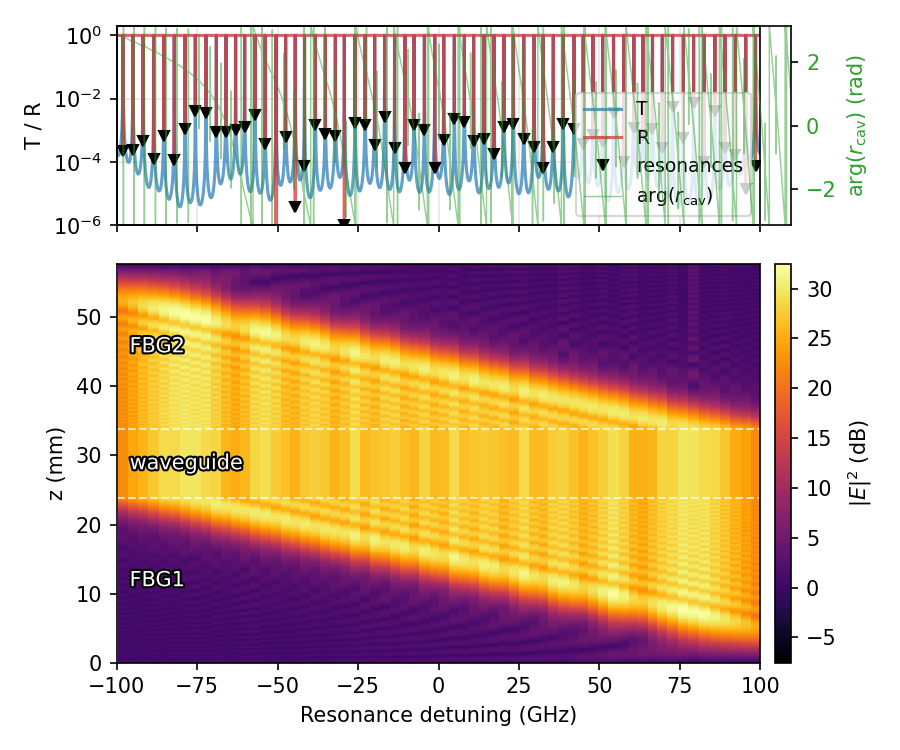
\includegraphics[width=0.95\linewidth]{fig/cavity_intra_010.png}
  \caption{Top: cavity transmission $T$ and reflection $R$ versus detuning, with resonances marked; the phase $\mathrm{arg}(r_\mathrm{cav})$ is overlaid. Despite the finite frequency resolution, the cavity resonances (triangles) are reliably identified and used for the intracavity reconstruction. Bottom: reconstructed intracavity intensity envelope $|E|^2$ (dB) evaluated at the cavity resonances and plotted as a function of position $z$, showing field buildup across FBG1–waveguide–FBG2.}
  \label{fig:cavity_intra}
\end{figure}

% \paragraph{Top panel: spectrum and phase.}
% The dual $y$-axis layout follows the same idea as the single-FBG plot in
% \texttt{plot\_spectral\_phase\_shift.py}: amplitudes on a logarithmic
% left axis, phase on a linear right axis. The phase is drawn wrapped,
% $\arg r_\mathrm{cav} \in [-\pi,\pi]$, so each high-finesse cavity resonance
% appears as a near-vertical $\sim 2\pi$ wind around the corresponding $R$
% minimum. Resonance markers are placed at $|r_\mathrm{cav}(\nu_p)|^2$ rather
% than at a fixed height, so they trace the local minima of the $R$ curve.

% \paragraph{Bottom panel: intracavity buildup vs.\ $z$.}
% Each column is the standing-wave envelope along $z$ at one resonance
% frequency. Inside the FBG zones, $|E_\mathrm{env}|^2$ decays exponentially
% into the grating with the local Bragg penetration depth (which is itself
% frequency-dependent for a chirped grating, so the column profiles shift with
% $\nu$). Inside the waveguide zone, $|E_\mathrm{env}|^2$ is approximately
% spatially uniform at the cavity buildup factor; the colour bar reads the
% buildup directly relative to unit incident intensity.

% \paragraph{Geometric parameters at a glance.}
% \begin{itemize}\setlength\itemsep{2pt}
%   \item $L_\mathrm{FBG} = \sum_j a_j$: total chirped-grating length
%         (\texttt{nmax} cells, lattice profile \texttt{a\_in}).
%   \item $L_\mathrm{wg}$: waveguide length between the two FBGs
%         (\texttt{L\_wg}; default $10\,\mathrm{mm}$).
%   \item $n_\mathrm{wg}$: waveguide refractive index
%         (\texttt{n\_wg}; default $1.454$, matched to the FBG background
%         index $n_0$).
%   \item $\eta = $ \texttt{loss\_per\_pass}: fractional intensity loss for a
%         single pass through the waveguide (default $0$, lossless).
%   \item $\nu_0 = c/(1389\,\mathrm{nm})$: optical resonance frequency,
%         matching \texttt{gen\_fbg\_data.py}.
% \end{itemize}

% \section{HDF5 output}
% \label{sec:hdf5}

% \texttt{save\_cavity\_peaks} writes a peak-resolved file
% \texttt{data/cavity/cavity\_peaks\_\#NNN.hdf5} with the run parameters in the
% root attributes (\texttt{source}, \texttt{L\_wg\_m}, \texttt{n\_wg},
% \texttt{loss\_per\_pass}) and the following datasets:

% \begin{table}[h]
% \centering
% \begin{tabular}{lll}
% \toprule
% Dataset & Shape & Meaning \\
% \midrule
% \texttt{peak\_det} & $(P,)$ & resonance detuning $\delta_p = \nu_p - \nu_0$ in Hz \\
% \texttt{t\_fbg}, \texttt{r\_fbg} & $(P,)$ complex & single-FBG response at each peak \\
% \texttt{t\_cav}, \texttt{r\_cav} & $(P,)$ complex & cavity response at each peak \\
% \texttt{z\_um} & $(Z,)$ & axial-position grid in micrometres \\
% \texttt{intra} & $(Z, P)$ & $|E_\mathrm{env}(z_i, \nu_p)|^2$ \\
% \bottomrule
% \end{tabular}
% \end{table}

% \appendix

% \section{Standing-wave envelope identity}
% \label{app:envelope}

% For complex amplitudes $A,B \in \mathbb{C}$ and real phase $\theta$,
% \begin{align}
%   \bigl|A + B\,e^{i\theta}\bigr|^2
%   &= |A|^2 + |B|^2 + 2\,\Re\!\left(A^*\,B\,e^{i\theta}\right) \nonumber\\
%   &= |A|^2 + |B|^2 + 2\,|A|\,|B|\,\cos\!\bigl(\theta - \arg(A^*B)\bigr).
% \end{align}
% The maximum over $\theta$ is attained at $\theta = \arg(A^*B)$ and equals
% \begin{equation}
%   \max_{\theta}\bigl|A + B\,e^{i\theta}\bigr|^2
%   = |A|^2 + |B|^2 + 2\,|A|\,|B|
%   = \bigl(|A| + |B|\bigr)^2.
% \end{equation}
% Substituting $A = E_+(z)$, $B = E_-(z)$ and $\theta = 2\beta z$ gives
% Eq.~\eqref{eq:envelope}; sampling $|E|^2$ on a coarse $z$-grid that does not
% resolve the rapid $2\beta z$ phase therefore underestimates the true peak
% intensity by exactly the amount we recover by recording the closed-form
% envelope $(|E_+|+|E_-|)^2$.

\begin{thebibliography}{99}


\bibitem{Erdogan1997}
T.~Erdogan, Fiber grating spectra, J. Lightwave Technol. \textbf{15}, 1277 (1997).

\bibitem{OthonosKalli1999}
A.~Othonos and K.~Kalli, \textit{Fiber Bragg Gratings: Fundamentals and Applications in Telecommunications and Sensing} (Artech House, Boston, 1999).

\bibitem{Kashyap2009}
R.~Kashyap, \textit{Fiber Bragg Gratings}, 2nd ed. (Academic Press, San Diego, 2009).

\bibitem{YarivYeh1984}
A.~Yariv and P.~Yeh, \textit{Optical Waves in Crystals} (Wiley, New York, 1984).

\bibitem{Joannopoulos2008}
J.~D. Joannopoulos, S.~G. Johnson, J.~N. Winn, and R.~D. Meade, \textit{Photonic Crystals: Molding the Flow of Light}, 2nd ed. (Princeton University Press, Princeton, 2008).

\bibitem{Markos2008}
P. Markoš and C. M. Soukoulis,
\textit{Wave Propagation: From Electrons to Photonic Crystals and Left-Handed Materials}
(Princeton University Press, 2008).

\bibitem{1dfbgnote}
Internal note, \textit{Note on 1D model of an FBG cavity and temperature sensitivity}
\end{thebibliography}
\end{document}
